%%%%%%%%%%%%%%%%%%%%%%%%%%%%%%%%%%%%%%%%%
% baposter portrait Poster - modified by Irina Wagner, bluezouzou@gmail.com, July 2016.
% LaTeX Template
% Version 1.0 (11/06/13)
%
% baposter Class Created by:
% Brian Amberg (baposter@brian-amberg.de)
%
% This template has been downloaded from:
% http://www.LaTeXTemplates.com
%
% License:
% CC BY-NC-SA 3.0 (http://creativecommons.org/licenses/by-nc-sa/3.0/)
%
%%%%%%%%%%%%%%%%%%%%%%%%%%%%%%%%%%%%%%%%%

%----------------------------------------------------------------------------------------
%	PACKAGES AND OTHER DOCUMENT CONFIGURATIONS
%---------------------------------------------------------------------------------------


\documentclass[portrait,a0paper,fontscale=0.36]{baposter} % Adjust the font scale/size here

\usepackage{graphicx} % Required for including images
\graphicspath{{figures/}} % Directory in which figures are stored
\usepackage[scaled=.92]{helvet}
\renewcommand{\familydefault}{\sfdefault}

\usepackage{natbib}

\usepackage{amsmath} % For typesetting math
\usepackage{amssymb} % Adds new symbols to be used in math mode
\usepackage{booktabs} % Top and bottom rules for tables
\usepackage{enumitem} % Used to reduce itemize/enumerate spacing
\usepackage[font=small,labelfont=bf]{caption} % Required for specifying captions to tables and figures
\usepackage{changepage} %To adjust width
\usepackage{multicol} % Required for multiple columns
\setlength{\columnsep}{1.5em} % Slightly increase the space between columns
\setlength{\columnseprule}{0mm} % No horizontal rule between columns

\newcommand{\compresslist}{ % Define a command to reduce spacing within itemize/enumerate environments, this is used right after \begin{itemize} or \begin{enumerate}
\setlength{\itemsep}{1pt}
\setlength{\parskip}{0pt}
\setlength{\parsep}{0pt}
}

\setlist[itemize,1]{leftmargin=0.2in}
\setlist[itemize,2]{leftmargin=0.15in}

\setlist[enumerate,1]{leftmargin=0.25in}

\definecolor{lightgray}{HTML}{A2A4A3} % Defines the color used for content box headers
\definecolor{cublack}{HTML}{000000}
\definecolor{cugold}{HTML}{cccc66}
\usepackage{tikz-dependency}
\usepackage{gb4e}

\begin{document}

\begin{poster}
{
headerborder=closed, % Adds a border around the header of content boxes
colspacing=1em, % Column spacing
bgColorOne=white, % Background color for the gradient on the left side of the poster
bgColorTwo=white, % Background color for the gradient on the right side of the poster
borderColor=cublack, % Border color
headerColorOne=cublack, % Background color for the header in the content boxes (left side)
headerColorTwo=cublack, % Background color for the header in the content boxes (right side)
headerFontColor=cugold, % Text color for the header text in the content boxes
boxColorOne=white, % Background color of the content boxes
textborder=roundedleft, % Format of the border around content boxes, can be: none, bars, coils, triangles, rectangle, rounded, roundedsmall, roundedright or faded
eyecatcher=true, % Set to false for ignoring the left logo in the title and move the title left
headerheight=0.1\textheight, % Height of the header
headershape=roundedright, % Specify the rounded corner in the content box headers, can be: rectangle, small-rounded, roundedright, roundedleft or rounded
headerfont=\Large\bf, % Large, bold and sans serif font in the headers of content boxes
%textfont={\setlength{\parindent}{1.5em}}, % Uncomment for paragraph indentation
linewidth=1pt % Width of the border lines around content boxes
}
%----------------------------------------------------------------------------------------
%	TITLE SECTION 
%----------------------------------------------------------------------------------------
%
{
\includegraphics[height=8em]{culogo.png}}
{\textbf{\huge Applying Universal Dependency  to the Arapaho Language \vspace{0.1em}
}\vspace{0.15em}} % Poster title
{Irina Wagner\textsuperscript{1}, Andrew Cowell\textsuperscript{1}, Jena D. Hwang\textsuperscript{2} \\
\hspace{6pt}\hspace{6pt}\textsuperscript{1}University of Colorado Boulder,
  Department of Linguistics; \textsuperscript{2}IHMC\\
  \vspace{0.05in} \small {\tt \{irina.wagner, james.cowell\}@colorado.edu,  jhwang@ihmc.us}} % Author names and institution
{
\includegraphics[height=3em]{ihmc.png}} % Second university/lab logo on the right

%----------------------------------------------------------------------------------------
%	OBJECTIVES
%----------------------------------------------------------------------------------------

\headerbox{Objectives}{name=objectives,column=0,row=0}{

Although Universal Dependency scheme is both comprehensive and eloquent, it also assumes certain grammatical structures to be cross-linguistically universal.  In our project :
\begin{itemize}\compresslist
\item we \textbf{demonstrate the applicability} of these assumptions to annotations of the Arapaho language;
\item and \textbf{propose language-specific guidelines} to account for particular features of Algonquian syntax.
\end{itemize}
}
%----------------------------------------------------------------------------------------
%	ARAPAHO
%----------------------------------------------------------------------------------------

\headerbox{Arapaho Language}{name=arapaho,column=0,below=objectives}{
\begin{multicols}{2}
\captionof{figure}{Traditional Arapaho territory}
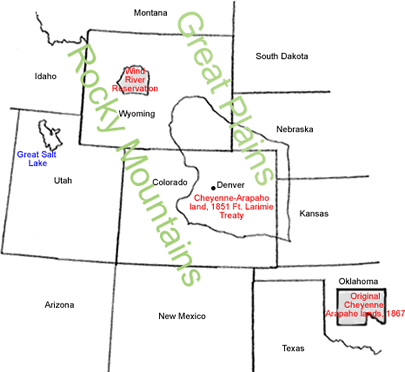
\includegraphics[scale=0.3]{Arapahomap}


\begin{itemize} \compresslist
\item Algonquian.
\item Poly-synthetic agglutinating language.
\item Critically endangered.
\item Spoken in Wind River Indian Reservation in Wyoming, USA.
\item Available transcribed and translated spoken corpus.
\end{itemize}
\end{multicols}
}
%----------------------------------------------------------------------------------------
%	FEATURES
%----------------------------------------------------------------------------------------

\headerbox{Problematic Features of Arapaho}{name=features,column=0,below=arapaho}{ % This block's bottom aligns with the bottom of the conclusion block

\textbf{Verbal Complexity}
\vspace{-0.75em}
	\begin{itemize}\compresslist
		\item he'ih'ii-xoo-xook-bix-ohoe-koohuut-oo-no'\\
\textit{``Their hands would go right through them and appear on the other side.''}
	\end{itemize}
\textbf{Transitivity}
\vspace{-0.75em}

	\begin{itemize}\compresslist
		\item Difference in syntactic and semantic transitivity is reflected in verbal morphology \cite{Cow08}.
		\item All of the verbs may have two nominals they seem to agree with in meaning or none at all.
\begin{multicols}{2} \footnotesize
\begin{adjustwidth*}{-0.3in}{-0.3in}
\begin{exe}
\ex
\gll nih-to'ow-oot.\\
{\textsc{pst}-hit-\textsc{3s/4}}\\
\trans \textit{``S/he hit him/her''}
\end{exe}
\end{adjustwidth*}
\vfill \columnbreak
\begin{adjustwidth*}{-0.65in}{-0.65in}
\begin{exe}
\ex
\gll nih-'iikooko'uyei-3i' biino.\\
{\textsc{pst}-pick things-\textsc{3pl}} chokecherries\\
\trans \textit{``They picked chokecherries''}
\end{exe}
\end{adjustwidth*}
\normalsize
		\end{multicols}
	
	\end{itemize}
\textbf{Obviation}
\begin{itemize}\compresslist
	\item When two or more third person animate nouns are present, one of them, the less pragmatically important one \cite{Goddard1984}, is marked obviative, the verb agreeing with such noun is also marked.
	
	\footnotesize
	\begin{adjustwidth*}{-0.3in}{-0.3in}
\begin{exe}
\ex \label{obviation}
\gll {hee3\textbf{eihok}} {\textbf{hiinoon}} {3eeyokooxuu}.\\
{say to s.o.-\textsc{4/3s.subj}} {his/her mother} {Tipi-pole Child} \\
\trans \textit{His mother said to Under-the-Tipi-Pole Child.}
\end{exe}
\end{adjustwidth*}
\normalsize
	
\end{itemize}
}
%----------------------------------------------------------------------------------------
%	ANNOTATIONS
%----------------------------------------------------------------------------------------

\headerbox{Annotations}{name=annotations,column=0,below=features}{ % This block's bottom aligns with the bottom of the conclusion block
\begin{itemize}\compresslist
\item Manual annotations by graduate students in Linguistics. 
\item Kept in spreadsheet format.
\item Checked by a fluent non-native speaker.
\item Two phases of annotations:

Phase 1: \textbf{Initial annotations of traditional narratives.}
\begin{itemize}\compresslist
\small \item About 2,000 lines.
\item Patterns of Algonquian syntax used for the guidelines.
\end{itemize}

\normalsize
Phase 2: \textbf{Additional narratives and conversations.}
	\begin{itemize}\compresslist
\small 	\item Stanford Dependencies \cite{Marneffe2008} used as the base, annotations converted.
		\item + 3616 lines of elicited personal and traditional oral narratives 
		\item + 593 lines of conversational data.
		\item Universal Dependency \cite{ud2014} is adopted to account for conversational disfluencies.
		\item Previous annotations were converted according to the \textsc{ud} scheme.
	\end{itemize}
\end{itemize}
}



%----------------------------------------------------------------------------------------
%	UD
%----------------------------------------------------------------------------------------

\headerbox{Mapping to the UD scheme}{name=ud,column=0,below=annotations, above=bottom}
{ \vspace{8px}
\begin{itemize}
\item Out of 40 \textsc{ud} dependencies, \textbf{30 have one-to-one correspondence}. For example, the adverbial clause dependency:
\footnotesize
\begin{exe}
\ex \label{advcl} %Con124.051
\begin{dependency}
\begin{deptext}
Bih'iyoohok \& ce'no'useeni'.\\
\textsc{vii} \& \textsc{vai}\\
\end{deptext}
\depedge [edge unit distance=1ex]{1}	{2}	{advcl}
\end{dependency}
\gll \textbf{Bih'iyoo-hok} ce'-no'usee-ni'.\\
{dark-\textsc{subjunct}} {back-arrive-\textsc{1pl}}\\
\trans \textit{``When it's dark, we'll come back.''}
\end{exe}

\normalsize
\item Added  \textbf{17 Arapaho-specific} dependencies.
\item Some dependencies were eliminated because they do not exist (e.g., \textit{xcomp, neg, amod, nummod, aux, auxpass, cop, expl, mark, mwe}).
\end{itemize}
}
%----------------------------------------------------------------------------------------
%	SUBJECTS
%----------------------------------------------------------------------------------------
\headerbox{Subjects}{name=subjects,column=1,row=0}
{
\begin{itemize}\compresslist
\item Subjects are not distinguished syntactically by word order. 
\item Obviation by itself also does not specify syntactic dependency but disambiguates between nominals.
\item Only intransitive animate (\textsc{vai}), intransitive inanimate (\textsc{vii}) and transitive inanimate verbs (\textsc{vti}) exhibit agreement with syntactic subjects. 
\small
\begin{exe}
\ex \label{nsubj:obv} %Con109.064
\begin{dependency}
\begin{deptext}
no'useeni3 \& nuhu' \& koo'ohwuu.\\
\textsc{vai} \& \textsc{det} \& \textsc{na}\\
\end{deptext}
\depedge [edge unit distance=1ex]{3}	{1}	{nsubj:obv}
\end{dependency}
\gll no'usee-ni3 nuhu' \textbf{koo'ohw-uu}.\\
{arrive-\textsc{4s}} this coyote-obv.\\
\trans \textit{``This coyote came.''}
\end{exe}
\normalsize
\item Because transitive animate verbs (\textsc{vta}) are marked for obviation and the direction of action, the agent distinction (\textit{nagent(:obv)}) is used instead:
\small
\begin{exe}
\ex \label{agent:obv}%con3.137
\begin{dependency}
\begin{deptext}
hiniisonoon \& heenei'itowuuneit.\\
\textsc{na} \& \textsc{vta}\\
\end{deptext}
\depedge[edge unit distance=1.5ex]{1}	{2}	{nagent:obv}
\end{dependency}
\gll \textbf{hi-niisonoon} {heen-ei'itowuun-eit}.\\
\textsc{3s}-father.obv {\textsc{redup}-tell s.o.-\textsc{4/3s}}\\
\trans \textit{His father tells him.}
\end{exe}
\normalsize
\item When transitive verbs passivized, semantic agents may remain in the clause as obliques (\textit{nagent:oblique}):
 \small
\begin{exe}
\ex \label{middle}
\begin{dependency}
\begin{deptext}
Neisonoo \& nihcihwonbiineihini3i \& nebesiiwoho'.\\
\textsc{na} \& \textsc{vai.pass}	\& \textsc{na}\\
\end{deptext}
\depedge [edge unit distance=1.5ex]{1}{2}{nagent:oblique}
\depedge[edge unit distance=1ex]{3}	{2}	{nsubjpass:obv}
\end{dependency}
\begin{adjustwidth*}{-0.6in}{-0.6in}
\gll \textbf{ne-isonoo} {nih-cih-won-biin-\textbf{eihi-ni3i}} {ne-besiiwoho'} \\
\textbf{\textsc{1s}-father} {\textsc{pst}-to here-\textsc{allat}-give-\textsc{pass}-\textsc{4pl}} \textsc{1s}-grandfathers.obv\\
\trans \textit{``My grandfathers were given (sth) by my father''}
\end{adjustwidth*}
\end{exe}
\normalsize
\end{itemize}
}
%----------------------------------------------------------------------------------------
%	OBJECTS
%----------------------------------------------------------------------------------------
\headerbox{Objects}{name=objects,column=1,row=2,below=subjects}
{
\begin{itemize} \compresslist
\item Almost any semantic role can be expressed by an ``object.''
\item Any ``classic'' object can be demoted and not marked verbally.
\item Overt nominal expressions of an object are not always necessary.
\item The only true direct object is the inanimate object of a \textsc{vti}:

\small
\begin{exe}
\ex \label{objct} %con15.014
\begin{dependency}
\begin{deptext}
niico'ontonounowoo \& nuhu' \& niinen.\\
\textsc{vti} \& \textsc{det} \& \textsc{ni}\\
\end{deptext}
\depedge [edge unit distance=1ex]{3}	{1}	{dobj}
\end{dependency}
\gll nii-co'on-tonoun-owoo nuhu' \textbf{niinen}.\\
{\textsc{impf}-always-use-\textsc{1s}} this {piece of fat}\\
\trans \textit{``I always use this fat.''}
\end{exe}
\normalsize
\item Ditransitive constructions verbally mark only animate nominals, so the overt inanimate nominal is actually an indirect object: 

\small
\begin{exe}
\ex \label{objse} %con110.060
\begin{dependency}
\begin{deptext}
Cihneeneeciihi \& hesiiseii.\\
\textsc{vta} \& \textsc{ni} \\
\end{deptext}
\depedge [edge unit distance=1ex]{2}{1}	{iobj}
\end{dependency}
\gll Cih-nee-neeciih-i \textbf{he-siiseii}\\
{\textsc{emph.imper-redup}-lend-\textsc{1s.imper}} {\textsc{2s}-eyes}\\
\trans \textit{``Lend me your eyes.''}
\end{exe}
\normalsize
\item Semantic label ``undergoer'' is used to further specify the direct objects of transitive animate verbs: 

\footnotesize
\begin{exe}
\ex \label{under}
\begin{dependency}
\begin{deptext}
Neisonoo \& nihcihwonbiinoot \& nebesiiwoho'.\\
\textsc{na} \& \textsc{vta}	\& \textsc{na}\\
\end{deptext}
\depedge [edge unit distance=1.5ex]{1}{2}{nsubj:agent}
\depedge[edge unit distance=1ex]{3}	{2}	{dobj:under:obv}
\end{dependency}
\begin{adjustwidth*}{-0.5in}{-0.5in}
\gll \textbf{ne-isonoo} {nih-cih-won-biin-oot} \textbf{ne-besiiwoho'} \\
\textbf{\textsc{1s}-father} {\textsc{pst}-to here-\textsc{allat}-give-\textsc{3s/4}} \textbf{\textsc{1s}-grandfathers.obv}\\
\trans \textit{``My father came to give [me] to my grandfather.''}
\end{adjustwidth*}
\end{exe}

\normalsize
\end{itemize}
}
%----------------------------------------------------------------------------------------
%	NVR
%----------------------------------------------------------------------------------------
\headerbox{Non-Verbal Roots}{name=nvr,column=1,row=3, below=objects, above=bottom}
{\vspace{8px}
\begin{itemize} 
\item \textit{root} is a pragmatically independent word, not a particular part of speech.
\item In predicative constructions, the \textit{root} is the topic, while the predicate is labeled as \textit{backreference}
\begin{exe}
\ex \label{topic}
\footnotesize
\begin{dependency}
\begin{deptext}
Ni'ook \& he'ne'nih'iisih'it.\\
\textsc{name} \& \textsc{vai.pass}\\
\end{deptext}
\deproot [edge unit distance=1.5ex]{1}{root}
\depedge {2}{1}{backref}
\end{dependency}
\gll \textbf{{Ni'ook}} {he'ne'-nih-'iisih'i-t}\\
\textbf{{Puffy Eyes}} {that-\textsc{pst}-how named-\textsc{3s}}\\
\trans \textit{``Puffy Eyes, that is how he is named.''}

\end{exe}
\normalsize

\end{itemize}
}


%----------------------------------------------------------------------------------------
%	NMOD
%----------------------------------------------------------------------------------------
\headerbox{Noun Modifiers}{name=nmod,column=2,row=0}
{
\begin{itemize} \compresslist
\item \textit{nmod} relation is used to disambiguate between objects of transitive verbs and objects of intransitive verbs. 
\small
\begin{exe}
\ex \label{handgame} 
\begin{dependency}
\begin{deptext}
Ceebe'eiheinoo \& koxouhtiit\\
\textsc{vta}\& \textsc{ni}\\
\end{deptext}
\depedge [edge unit distance=1.5ex]{2}{1}{nmod}
\end{dependency}
\gll ceebe'eih-einoo \textbf{koxouhtiit}.\\
\textsc{ic}.beat-\textsc{3s/1s} handgame\\
\trans \textit{``He beats me in handgame.''}
\end{exe}
\normalsize
\item Specification \textit{:objim} (implied object) is used with objects of semi-transitive verbs:

\small
\begin{exe}
\ex \label{nmod:objim}%con123.006
\begin{dependency}
\begin{deptext}
neeyeih'oonotooneenou'u \& bei'ci3ei'i.\\
\textsc{vai.o}\& \textsc{ni}\\
\end{deptext}
\depedge {2}{1}{nmod:objim}
\end{dependency}
\gll neeyeih-'oonotoonee-nou'u \textbf{bei'ci3ei'i}.\\
{\textsc{ic}.try-\textsc{redup}-borrow things-12.\textsc{iter}} money\\
\trans \textit{``Whenever we try to borrow money.''}
\end{exe}
\normalsize
\item Implied and incorporated objects can be modified by an adverbial participle, like prepositions, and are labeled as \textit{:objad} -- object of an adverbial:

\small
\begin{exe}
\ex \label{objad}
\begin{dependency}
\begin{deptext}
nih'iinou'oo3i' \& neci' \& hi3oobei'i'\\
\textsc{vai}\& \textsc{na} \& \textsc{part}\\
\end{deptext}
\depedge {3}{2}{case}
\depedge{2}{1}{nmod:objad}
\end{dependency}
\gll nih-'iinou'oo-3i' \textbf{nec-i'} \textbf{hi3oobei'-i'}\\
{\textsc{pst}-float around-\textsc{3pl}} \textbf{water-\textsc{loc}} \textbf{{under sth-\textsc{loc}}}\\
\trans \textit{``They were floating around under the water''}
\end{exe}
\normalsize
\item \textit{nmod:instr} (instrumentals) are introduced by instrumental verbal prefixes and corresponding particles: \textit{hi'-, nohk-,} and \textit{nii3-}.
\item \textit{nmod:poss} marks the possessor:

\footnotesize
\begin{exe}
\ex \label{poss}
\begin{dependency}
\begin{deptext}
nii'ehihi' \& hi-siiseii\\
\textsc{na}\& \textsc{ni}\\
\end{deptext}
\depedge{1}{2}{nmod:poss}
\end{dependency}
\gll \textbf{nii'eihihi'} {hi-siiseii}\\
{little bird} {3\textsc{s}-eyes}\\
\trans \textit{``Little bird's eyes''}
\end{exe}
\end{itemize}
}

%----------------------------------------------------------------------------------------
%	FUTURE RESEARCH
%----------------------------------------------------------------------------------------

\headerbox{Future Research}{name=future,column=2,row=3, below=nmod}{ % This block is as tall as the references block
\begin{itemize} \compresslist
\item More manual annotations of conversational data.
\item Double annotations to ensure inter-annotator agreement.
\item Developing \textsc{pos} and dependency correspondences.
\item Subject this scheme to machine learning.
\end{itemize}
}

%----------------------------------------------------------------------------------------
%	CONCLUSION
%----------------------------------------------------------------------------------------

\headerbox{Conclusions}{name=conclusion,column=2,row=4,below=future}{

\begin{enumerate}\compresslist
\item Dependencies of nominal arguments should not rely purely on syntax but also include semantics and pragmatics.
\item Under-specification of semantic relationship for Arapaho leads to misrepresentation of some dependency relationships.
\item The guidelines developed for the Arapaho language demonstrate the use of both the universal patterns of syntax and the language-specific ones.
\end{enumerate}

\nocite{ud2014,Marneffe2014,Cow08,McDonald2013,Nivre2015} 

}
%----------------------------------------------------------------------------------------
%	REFERENCES
%----------------------------------------------------------------------------------------
\headerbox{References}
{name=references, column=2, below=conclusion}{
\renewcommand{\refname}{\vspace{-0.8em}}
{\compresslist \scriptsize
\bibliography{usethis}
\bibliographystyle{abbrv}}
}


% {\begin{center}
% 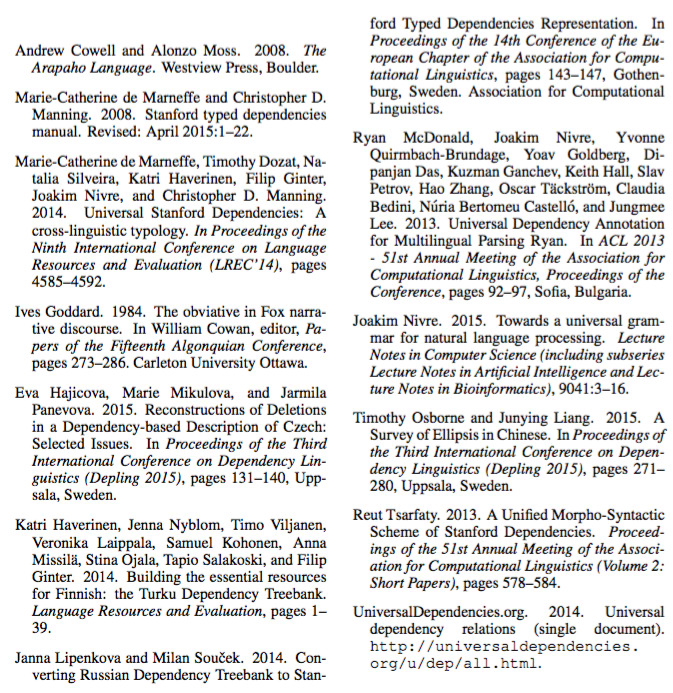
\includegraphics[scale=0.32]{references}
% \end{center}}
%----------------------------------------------------------------------------------------
% ACKNOWLEDGMENTS
%----------------------------------------------------------------------------------------
\headerbox{Acknowledgments}{name=acknowledgments,column=2,span=1, below=references,above=bottom}{ \vspace{10px}
The research is supported by the National Endowment for the Humanities grant, project number 1551671 ``Arapaho Lexical Database and Dictionary.'' We thank the Northern Arapaho tribe for allowing us to conduct the work with their language.
}


%----------------------------------------------------------------------------------------

\end{poster}

\end{document}